\part{First person camera control}
\frame{\partpage}

\begin{frame}{The plan}
	\begin{itemize}
		\pause\item Represent the player's \textbf{position} by a 3D vector
		\pause\item Represent the player's \textbf{orientation} by Euler angles
		\pause\item Mouse events change these angles
		\pause\item View matrix is calculated using position and orientation
		\pause\item To move forwards, use the Euler angles to find the ``forward'' vector,
			and offset the position by this vector
	\end{itemize}
\end{frame}

\begin{frame}{Keyboard and mouse in SDL}
	\pause Use \textbf{relative mouse mode}
	\begin{itemize}
		\pause\item Hides the mouse pointer
		\pause\item Prevents the mouse pointer from hitting the edge of the screen
		\pause\item Gives us the distance the mouse has moved since last frame, rather than its current position
	\end{itemize}
	\pause Use \lstinline{SDL_GetKeyboardState} instead of handling individual keyboard events
	\begin{itemize}
		\pause\item Allows us to check on every frame whether the key is held down
		\pause\item Otherwise, the player will move jerkily according to the key repeat rate
	\end{itemize}
\end{frame}

\begin{frame}{Vector addition}
	\pause
	\begin{center}
		\colorbox{white}{
			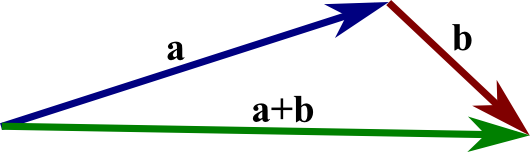
\includegraphics[width=0.5\textwidth]{vector_addition}
		}
	\end{center}
	\begin{itemize}
		\pause\item E.g.\ if $a$ is current position, and
		\pause\item $b$ is the distance and direction we want to move, then
		\pause\item $a + b$ is the new position
	\end{itemize}
\end{frame}

\begin{frame}{Addition in homogeneous coordinates}
	\begin{itemize}
		\pause\item Recall: homogeneous coordinates have an extra $w$ component, i.e.\ $(x,y,z,w)$
		\pause\item $w=1$ for positions, $w=0$ for offsets
	\end{itemize}
	\begin{tabular}{rclclc}
		\pause offset & + & offset & = & offset & $w = 0 + 0 = 0$ \\
		\pause position & + & offset & = & position & $w = 1 + 0 = 1$ \\
		\pause position & + & position & = & ??? & $w = 1 + 1 = 2$
	\end{tabular}
\end{frame}

\begin{frame}{Unit vectors}
	\begin{itemize}
		\pause\item A \textbf{unit vector} is a vector of length 1
		\pause\item I.e.\ $\sqrt{x^2 + y^2 + z^2} = 1$ (Pythagoras)
		\pause\item Useful to represent \textbf{direction}
		\pause\item Multiplying a vector of length $a$ by a number $b$ gives a vector of length $a \times b$,
			parallel to the original vector
		\pause\item So multiplying a unit vector by $b$ gives a vector of length $b$,
			parallel to the unit vector		
	\end{itemize}
\end{frame}

\begin{frame}{Representing look direction}
	\begin{columns}
		\pause
		\begin{column}{0.48\textwidth}
			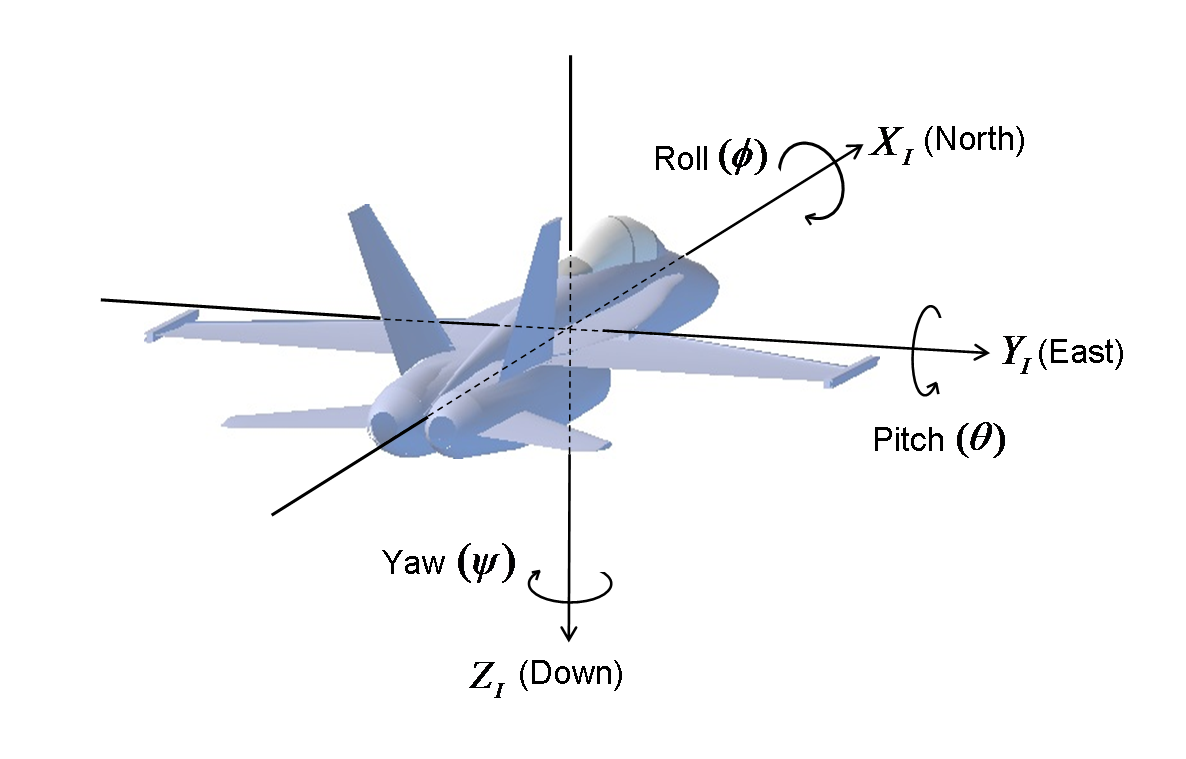
\includegraphics[width=\textwidth]{../03/euler_aeroplane}
		\end{column}
		\begin{column}{0.48\textwidth}
			\begin{itemize}
				\pause\item Euler angles
				\pause\item Don't need roll, just pitch and yaw
				\pause\item (Not using roll eliminates the gimbal lock problem)
				\pause\item Forward vector and look vector can be obtained by appropriate rotation of a unit vector
			\end{itemize}
		\end{column}
	\end{columns}
\end{frame}
